% Created 2017-11-29 Wed 17:00
\documentclass[11pt]{article}
\usepackage[utf8]{inputenc}
\usepackage[T1]{fontenc}
\usepackage{fixltx2e}
\usepackage{graphicx}
\usepackage{longtable}
\usepackage{float}
\usepackage{wrapfig}
\usepackage{soul}
\usepackage{textcomp}
\usepackage{marvosym}
\usepackage{wasysym}
\usepackage{latexsym}
\usepackage{amssymb}
\usepackage{hyperref}
\tolerance=1000
\providecommand{\alert}[1]{\textbf{#1}}

\title{correlation}
\author{secolinsky}
\date{\today}
\hypersetup{
  pdfkeywords={},
  pdfsubject={},
  pdfcreator={Emacs Org-mode version 7.9.3f}}

\begin{document}

\maketitle

\setcounter{tocdepth}{3}
\tableofcontents
\vspace*{1cm}
\section{Hypothesis Test}
\label{sec-1}

Goal is to calculate correlation coefficient and do the following
hypothesis test
\[ H_{0}: \rho = 0; H_{1} \rho \neq 0\]
using the data below

\begin{center}
\begin{tabular}{rr}
 age  &  price  \\
   5  &     85  \\
   4  &    103  \\
   6  &     70  \\
   5  &     82  \\
   5  &     89  \\
   5  &     98  \\
   6  &     66  \\
   6  &     95  \\
   2  &    169  \\
   7  &     70  \\
   7  &     48  \\
\end{tabular}
\end{center}



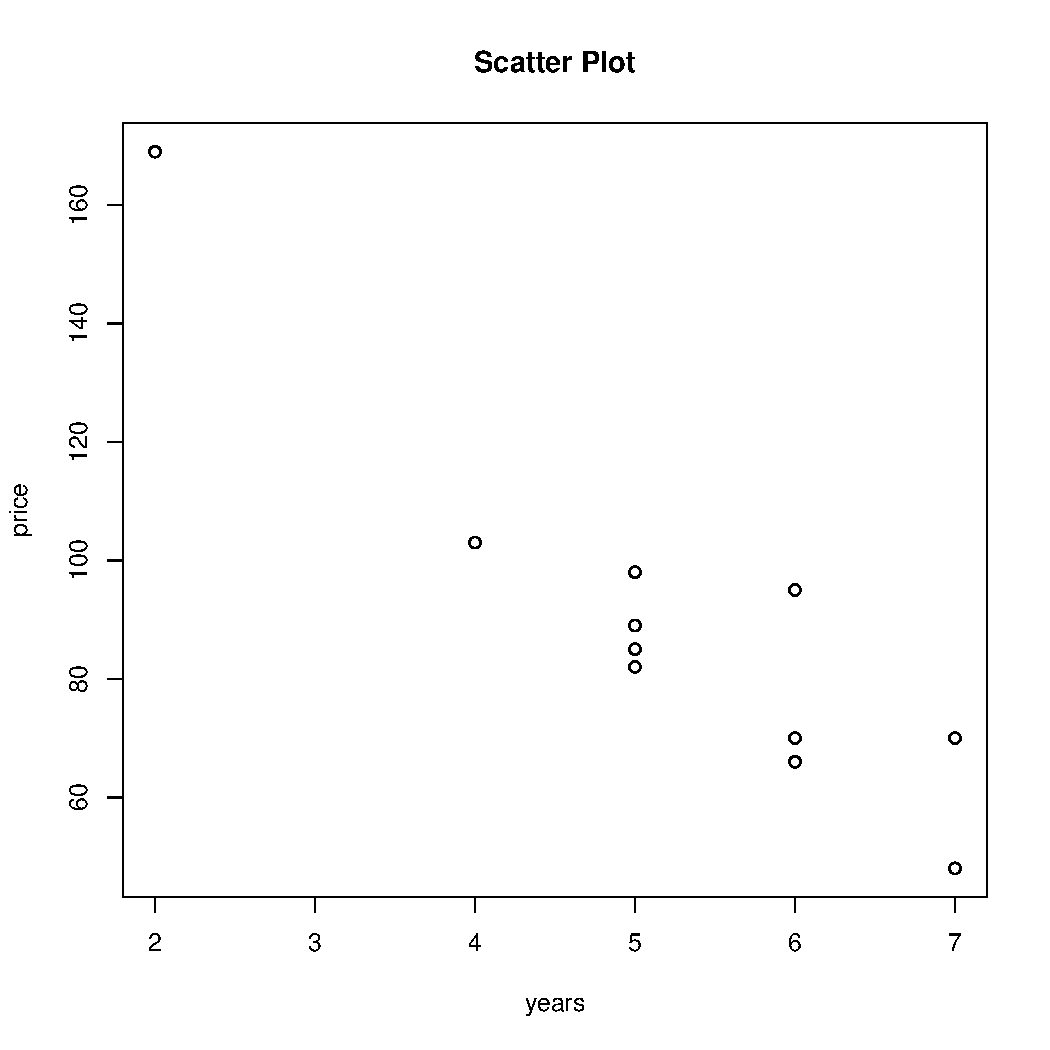
\includegraphics[scale=0.5]{scatter_plot.pdf}

From R we have that $\rho \approx -0.9804$ rounded to the fourth decimal place
and that the $p$-value \approx 0.00004882$.

For the linear regression model, we have that the y-intercept is 195.47
and the slope is -20.26.  To fit the model with the data, we use R to produce
the following graph:

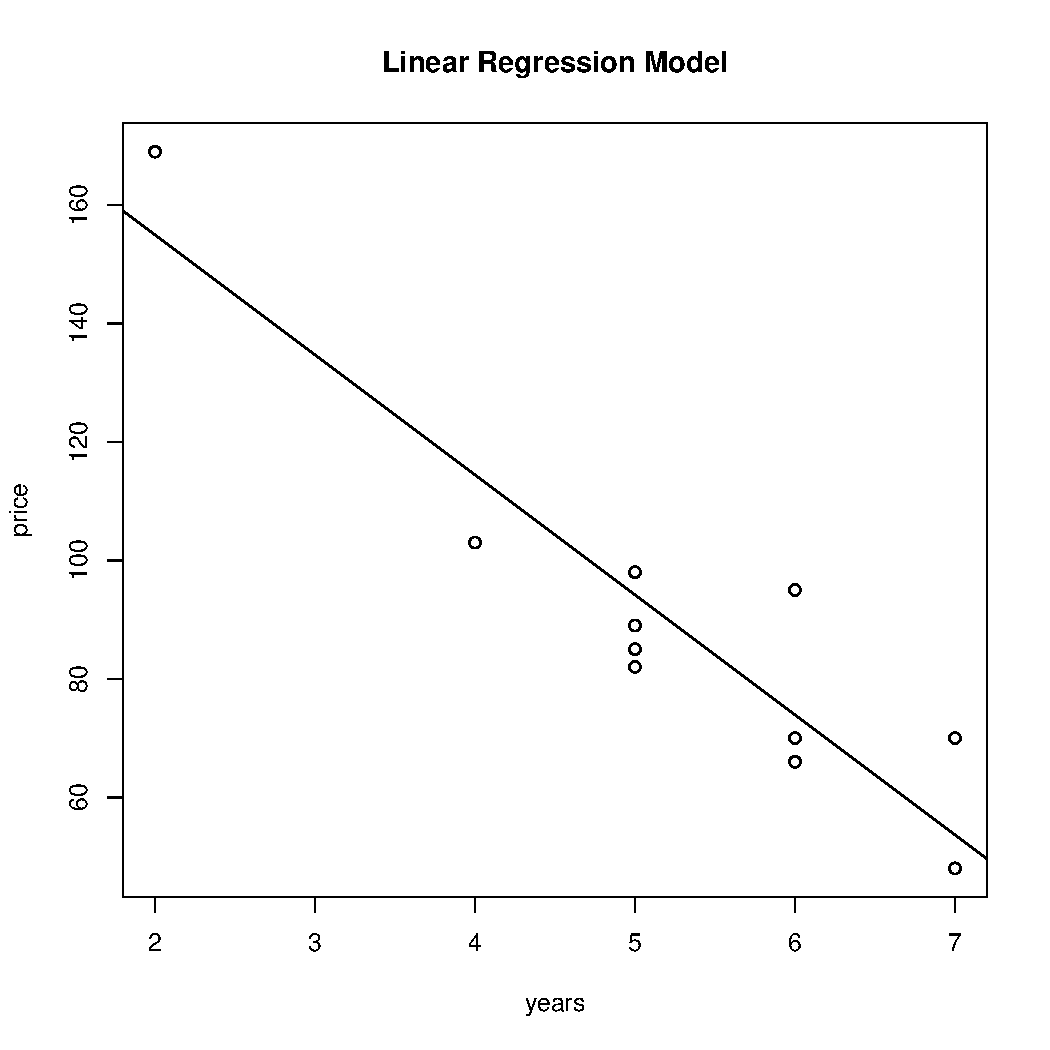
\includegraphics[scale=0.4]{regression_line.pdf}

\end{document}
